\newcommand{\examplescenescbar}{
	\begin{tikzpicture}[inner sep=0]
	\node(cbar){
\includegraphics[height=\size, width=2mm]{images/examples/inferno}};
	\node[xshift=1mm, anchor=north] at (cbar.north east){\tiny 1};
	\node[xshift=1mm, anchor=south] at (cbar.south east){\tiny 0};
	\end{tikzpicture}
}


% for text extending below like p, q, g
%\tikzset{
%	mylabel2/.style={
%		label={
%			[label distance=-1.25em, anchor=base]north:
%			\fcolorbox{black}{black}{
%				\scriptsize \color{tumgraylight} #1
%			}
%		}
%	}
%}

\newcommand{\tileexample}[9]{
\\ %% good classificaiton example
\node[inner sep=0]{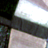
\includegraphics[width=\size]{images/examples/#1/rgb}}; \&
\node[inner sep=0]{
\includegraphics[width=\size]{images/examples/#1/ground_truth}}; \&
\node[inner sep=0]{
\includegraphics[width=\size]{images/examples/#1/prediction}}; \&
\node[inner sep=0]{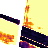
\includegraphics[width=\size]{images/examples/#1/masked_loss}}; \&
\node[inlabel=#3,inner sep=0]{\includegraphics[width=\size]{images/examples/#1/#2}}; \&
\node[inlabel=#5,inner sep=0]{\includegraphics[width=\size]{images/examples/#1/#4}}; \&
\node[inlabel=#7,inner sep=0]{\includegraphics[width=\size]{images/examples/#1/#6}}; \&
\node[inlabel=#9,inner sep=0]{\includegraphics[width=\size]{images/examples/#1/#8}}; \&
\examplescenescbar 	
}

%\\ %% good classificaiton example
%\node[rowlabel=A,inner sep=0]{
\includegraphics[width=\size]{images/examples/16494/rgb}}; \&
%\node[inner sep=0]{
\includegraphics[width=\size]{images/examples/16494/ground_truth}}; \&
%\node[inner sep=0]{
\includegraphics[width=\size]{images/examples/16494/prediction}}; \&
%\node[inner sep=0]{
\includegraphics[width=\size]{images/examples/16494/masked_loss}}; \&
%\node[inlabel=maize,inner sep=0]{
\includegraphics[width=\size]{images/examples/16494/maize}}; \&
%\node[inlabel=meadow,inner sep=0]{
\includegraphics[width=\size]{images/examples/16494/meadow}}; \&
%\node[inlabel=peas,inner sep=0]{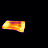
\includegraphics[width=\size]{images/examples/16494/peas}}; \&
%\node[inlabel=rape,inner sep=0]{
\includegraphics[width=\size]{images/examples/16494/rape}}; \&
%\examplescenescbar 	

\newcommand{\makeexamplelegend}{
\tiny
%\node[inner sep=0]{
\includegraphics[width=\size]{images/examples/color__asparagus}};
\matrix (n) [matrix of nodes, ampersand replacement=\&, row sep=0pt, column sep=2mm, below= 0mmof m]{
	\node[collabel=aspar., inner sep=0]{
\includegraphics[width=\colsize]{images/examples/color__asparagus}}; \&
	\node[collabel=bean,inner sep=0]{
\includegraphics[width=\colsize]{images/examples/color__beans}}; \&
	\node[collabel=hop,inner sep=0]{
\includegraphics[width=\colsize]{images/examples/color__hop}}; \&
	\node[collabel=maize,inner sep=0]{
\includegraphics[width=\colsize]{images/examples/color__maize}}; \&
	\node[collabel=mead.,inner sep=0]{
\includegraphics[width=\colsize]{images/examples/color__meadow}}; \&
	\node[collabel=peas,inner sep=0]{
\includegraphics[width=\colsize]{images/examples/color__peas}}; \&
	\node[collabel=pot.,inner sep=0]{
\includegraphics[width=\colsize]{images/examples/color__potatoe}}; \&
	\node[collabel=rape,inner sep=0]{
\includegraphics[width=\colsize]{images/examples/color__rape}}; \&
	\node[collabel=soyb.,inner sep=0]{
\includegraphics[width=\colsize]{images/examples/color__soybeans}}; \&
	\node[collabel=beet,inner sep=0]{
\includegraphics[width=\colsize]{images/examples/color__sugar_beet}}; \&
	\node[collabel=s.barl,inner sep=0]{
\includegraphics[width=\colsize]{images/examples/color__summer_barley}}; \&
	\node[collabel=oat,inner sep=0]{
\includegraphics[width=\colsize]{images/examples/color__summer_oat}}; \&
	\node[collabel=w.barl,inner sep=0]{
\includegraphics[width=\colsize]{images/examples/color__winter_barley}}; \&
	\node[collabel=rye,inner sep=0]{
\includegraphics[width=\colsize]{images/examples/color__winter_rye}}; \&
	\node[collabel=spelt,inner sep=0]{
\includegraphics[width=\colsize]{images/examples/color__winter_spelt}}; \&
	\node[collabel=tritic,inner sep=0]{
\includegraphics[width=\colsize]{images/examples/color__winter_triticale}}; \&
	\node[collabel=wheat,inner sep=0]{
\includegraphics[width=\colsize]{images/examples/color__winter_wheat}}; \&
	\\
};	
	
}

\tikzset{
	collabel/.style={
		label={
			[label distance=1.5em, anchor=base]south:
			\scriptsize \color{black} #1
		}
	}
}

\setlength{\fboxsep}{1pt}
\tikzset{
	inlabel/.style={
		label={
			[label distance=-1em, anchor=base]north:
			\fcolorbox{black}{black}{
				\scriptsize \color{tumgraylight} #1
			}
		}
	}
}

\tikzset{
	rowlabel/.style={
		label={
			[label distance=.51em, anchor=north west]north west:
			\fcolorbox{white}{white}{
				\color{black} \textbf{ \scriptsize #1 }
			}
		}
	}
}

\def\size{1.4cm}
\def\colsize{5mm}

%\colsize
\small

\newcommand{\makeimage}{

\begin{tikzpicture}

\matrix (m) [matrix of nodes, ampersand replacement=\&, row sep=0pt, column sep=2mm]{
	$\V{x}_{RGB,t}$ \& labels $\V{y}$ \& pred. $\hat{\V{y}}$ \& loss $H(\V{y},\hat{\V{y}}$) \& activation \& activation \& activation \& activation
	\tileexample{16494}{maize}{maize}{meadow}{meadow}{peas}{peas}{rape}{rape}
%	\\ %% Good example with correct prediction, but some loss
	\tileexample{8133}{winter_spelt}{spelt}{winter_wheat}{wheat}{summer_barley}{s.barley}{maize}{maize}
%	\\ %% Good example, only one small field partly wrong classified
	\tileexample{1823}{meadow}{meadow}{winter_wheat}{wheat}{summer_oat}{oat}{maize}{maize}
	\\ %% narrow fields
	\tileexample{12894}{meadow}{meadow}{winter_wheat}{wheat}{potatoe}{potato}{maize}{maize}
	\tileexample{2550}{maize}{maize}{winter_wheat}{wheat}{summer_barley}{s.barley}{winter_barley}{w.barley}
%	\\ %% Good example, only one small field partly wrong classified
	\tileexample{2554}{maize}{maize}{winter_wheat}{wheat}{meadow}{meadow}{winter_barley}{w.barley}
%	\\ %% Exampe of a forrest, which us a unknown class!
	\tileexample{10791}{maize}{maize}{winter_wheat}{wheat}{meadow}{meadow}{winter_barley}{w.barley}
%	\\ %% sparse label feature map
	\tileexample{10792}{winter_rye}{rye}{winter_wheat}{wheat}{winter_triticale}{triticale}{summer_barley}{s.barley}
%	\\ %% one field completely wrong classified. one field uncertain
	\tileexample{10879}{winter_rye}{rye}{winter_triticale}{triticale}{summer_barley}{s.barley}{winter_barley}{w.barley}
%	\\ %% Multiple fields uncertain
	\tileexample{10969}{winter_wheat}{wheat}{winter_triticale}{triticale}{winter_rye}{rye}{rape}{rape}
	%% one field uncertain
	\tileexample{172}{winter_wheat}{wheat}{meadow}{meadow}{maize}{maize}{winter_barley}{w.barley}
	\\
};

\makeexamplelegend
\end{tikzpicture}

}